\documentclass[12pt]{article}
\usepackage[utf8]{inputenc}
\usepackage{blindtext}
\usepackage{fancyhdr}
\usepackage{graphicx}
\usepackage{amsmath}
\usepackage{amssymb}
\usepackage[table,xcdraw]{xcolor}
\usepackage{commath}
\usepackage{float}
  \usepackage{setspace}
\usepackage{geometry}
 \geometry{
 a4paper,
 left=20mm,
 right=20mm,
 bottom=25mm,
 top=25mm,
 }
 \usepackage[
backend=biber,
style=mla-new,
citestyle=authoryear
]{biblatex}
\addbibresource{sources.bib}
 
 \newcommand{\icol}[1]{% inline column vector
  \left(\begin{smallmatrix}#1\end{smallmatrix}\right)%
}
\pagestyle{fancy}
\fancyhf{}
\lhead{Research Question: How fast should a camera rotate to record a zipliner traveling at constant velocity in the center of the frame? }
\rfoot{Page \thepage}

\doublespacing
\begin{document}

\nocite{zippic}
\nocite{annotated}

\begin{titlepage}
   \begin{center}

        \Huge{Related Rates of a Camera Videotaping Zipliners}

        \vspace{0.5cm}
        \LARGE{How fast should a camera rotate to record a zipliner traveling at constant velocity in the center of the frame?}
        \vspace{0.5cm}
        \begin{figure}[H]
        \centering
        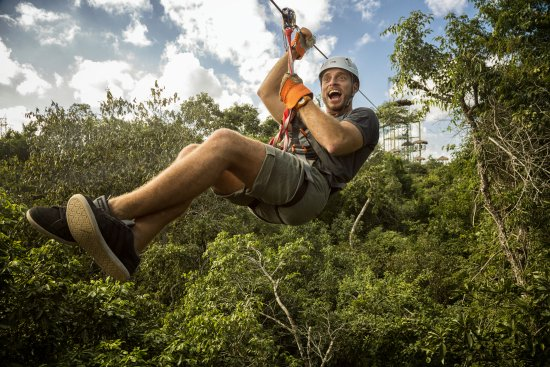
\includegraphics[width=400pt]{img/zipline.jpg}
        \caption{\label{fig:0} Photograph of Zipliner on Selvatica Zipline, Cancun ("Review...")}
        \end{figure}

        \vspace{0.5 cm}
        \Large{IB Code \#: jmy571}
        
        \vspace{1 cm}
        \large{18 Pages}
      
        \large{IB Mathematics Analysis and Approaches Higher Level}

        \Large{Internal Assessment}
       

       \vfill
    \end{center}
\end{titlepage}
    
\tableofcontents
\newpage
    
\section{Introduction}
My uncle owns a zipline park in Yucatan, Mexico, which is mostly visited by tourists for the stunning views. Tourists have often wanted to have videos taken of them, but there is currently no implementation of a camera to record them. Videos taken from stationary viewers often fail to smoothly track the motion of the zipliners, resulting in bad-quality videos and no memories from the zipline. I saw this as an opportunity to position mechanical motors rotating a camera which will change orientation over time to track and record the entire ride of the zipliners, from start to finish, as shown in Figure 1.

\begin{figure}[H]
\centering
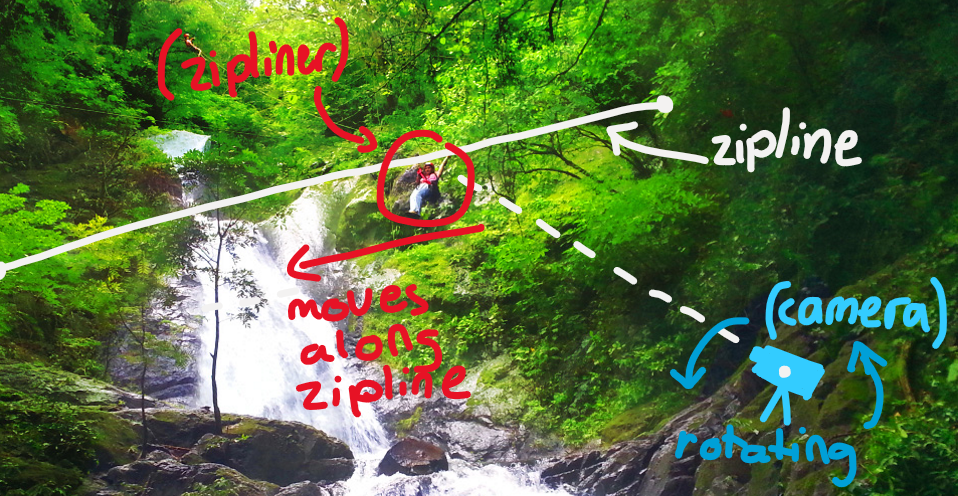
\includegraphics[width=500pt]{img/annotation.png}
\caption{\label{fig:1}Annotated Diagram of Camera Tracking Zipliner ("Mega...")}
\end{figure}

\subsection{Rationale}
This investigation seeks to find the rate at which the motors of the camera should rotate to track the zipliner as they descend from the start point to the finish point. I will use vectors to represent the three-dimensional zipline and the orientation of the camera in 3D space defined by two angles that will control the mechanical motors that spin the camera. To find how fast they should rotate, I will also have to apply differential calculus to find the rate of change of the angle of these motors on the camera. Since there are several ziplines at the park and many places to position the camera for different background views, I want to find a general solution to the rates of change of the angles for any zipline in the park with a camera at any point. I will then apply it to one of the smaller ziplines that has a beautiful view over a river. 

\subsection{Aim}
The aim of this investigation is to successfully study the influence of the position of a zipliner on the angle of rotation to design a device that will allow recording the experience in High Definition and always with the zipliner at the center of the frame for tourists to forever remember their zipline adventure with high quality videos to look back on. I will do so by answering the research question "How fast should a camera rotate to record a zipliner traveling at constant velocity in the center of the frame?" In answering this question, I will ultimately find equations for the rates of change of the angles defining the orientation of the camera over time as the zipliner travels down the zipline. 

\section{Defining the Problem}

I will position the camera next to the zipline on a stand at the same height as the end of the zipline, and want it to rotate in such a way that it tracks the zipliner as they descend. I will define the following variables in the table below, which are the given variables for any zipline. I have also found the values of each variable for the zipline I will be recording. 


In this scenario, I set up the camera as the origin, point $O(0,0,0)$, for improved readability when doing the calculations. This is because I am ultimately measuring all points in reference to the camera which is stationary, so it makes most sense to treat it as the origin and minimize unnecessary calculations. However, I want to have the possibility to change the camera's location, so I will still proceed by treating the origin and point $C$ as their own coordinates for future changes to the camera's position. I have also defined the orthogonal vectors $\vec i$, $\vec j$, as North-South and East-West, respectively (these will be the axis of the 3-dimensional space I will be analyzing), and $\vec k$ as the vertical height relative to the origin.

% variable stuff // meaning // application

\begin{table}[H]
\centering
\begin{tabular}{|l|l|l|}
\hline
\rowcolor[HTML]{C0C0C0} 
Variable     & Meaning                                                                                      & Real Value \\ \hline
$P_i(x_i,y_i,z_i)$ & \begin{tabular}[c]{@{}l@{}}Point where the zipline starts\\ and its coordinates in meters\end{tabular} & $P_i(24,28,11)$    \\ \hline
$P_f(x_f, y_f, z_f)$ & \begin{tabular}[c]{@{}l@{}}Point where the zipline ends \\ and its coordinates in meters\end{tabular}  & $P_f(-28,8,0)$  \\ \hline
$C(x_c, y_c, z_c)$ & \begin{tabular}[c]{@{}l@{}}Location of the camera \\ in meters\end{tabular}  &  $C(0,0,0)$  \\ \hline
$\vec v = v_x\vec i + v_y\vec j + v_z \vec k$ & \begin{tabular}[c]{@{}l@{}}Velocity vector of zipliner \\ assuming constant velocity \\ in meters per seconds squared \end{tabular}  &  $\vec v = -5.2\vec i - 2\vec j - 1.1 \vec k$  \\ \hline
$t$ & \begin{tabular}[c]{@{}l@{}}Time (in seconds) since \\ the zipliner began traveling \end{tabular}  &   \\ \hline
\end{tabular}
\end{table}


It would be helpful to find the coordinates of the point at which the zipliner is currently located as a function of time. Expressing this point, let's call it $P_c$, as a vector from the origin, $\overrightarrow{OP_c}$, we have the following equation for it using the line of the zipline, 

$$\overrightarrow{OP_c} = \begin{pmatrix} x_i \\ y_i \\ z_i \\ \end{pmatrix} + t\begin{pmatrix} v_x \\ v_y \\ v_z \\ \end{pmatrix}$$
Alternatively, we can express the coordinates of any point on the zipline as the current position, 
$$P_c(x_i+tv_x, y_i+tv_y, z_i+tv_z)$$


\section{Finding an Equation for Each Angle}

Now we can begin searching for equations defining the orientation of the camera. To do that, we first have to define what we mean by the camera 'following' the zipliner. This means that the camera will always be pointing at the zipliner, thus keeping them in the center of the frame at all times. This direction is defined by the vector between the points $C$ and $P_c$. Hence, we can define the following vector. For improved readability, I will call it $\vec n$.
$$\vec n = \overrightarrow{CP_c} = \begin{pmatrix} x_i + tv_x - c_x \\ y_i + tv_y - c_y \\ z_i + tv_z - c_z \\
\end{pmatrix} = \begin{pmatrix} x_t \\ y_t \\ z_t \\
\end{pmatrix}$$

Using this vector, I sketched the following diagram to visualize the problem.

\begin{figure}[H]
\centering
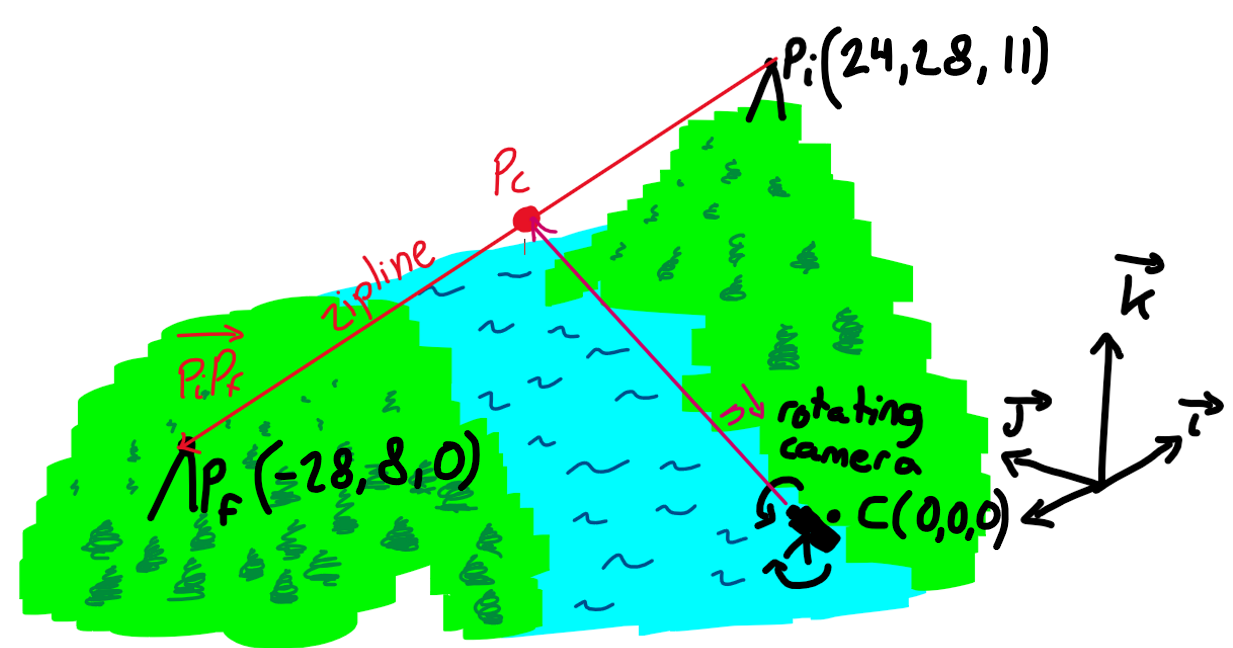
\includegraphics[width=450pt]{img/annotation1.png}
\caption{\label{fig:4}My Sketch of my Uncle's Zipline with Outlined Points and Vectors}
\end{figure}

Now that we know that by the camera's orientation is defined by the vector $\vec n$, let's find the angles that define the direction of this vector, in radians, which the mechanical motors will use to rotate such that they track the coordinate position of $P_c$. Since I ultimately want to find an angle, I will define the direction of the vector using the angles between it and the orthogonal vectors $\vec i$ and $\vec j$, which are also the x-axis and y-axis, respectively. I can then set up my motors to rotate the camera along those axis to follow the current position of the zipliner. To do that, let's define the unit vectors of each axis in the three dimensions, 


$$\vec i = \begin{pmatrix} 1 \\ 0 \\ 0 \\
\end{pmatrix}, \quad \vec j = \begin{pmatrix} 0 \\ 1 \\ 0 \\
\end{pmatrix}, \quad \vec k = \begin{pmatrix} 0 \\ 0 \\ 1 \\ \end{pmatrix}$$

Now, let's define the following angles which will be the focus of this investigation. We ultimately want to find their rates of change across time.
$$
\begin{array}{lc}
 \theta_x & \text{(Angle, in radians, between } \vec i \text{ and } \vec n \text{)}\\
 \theta_y & \text{(Angle, in radians, between } \vec j \text{ and } \vec n\text{)}\\
\end{array}
$$

I constructed the following diagram in Figure 3 to demonstrate the meaning of each angle. As shown, the angles define the orientation of the camera, and therefore will be used to position the camera in such a way that it follows the zipliner.

\begin{figure}[H]
\centering
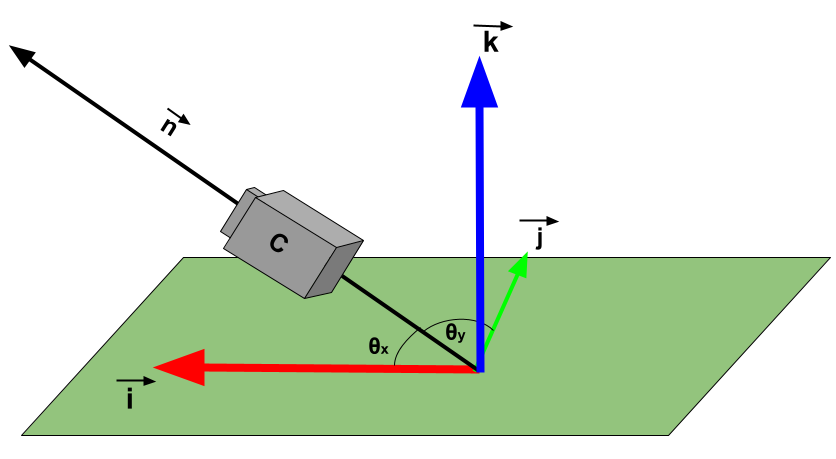
\includegraphics[width=400pt]{img/angles.png}
\caption{\label{fig:2}Diagram of Camera's Rotation Angles with Orthogonal Vectors}
\end{figure}

To find these angles, I will use the scalar product between the line of sight of the camera, $\vec n$, and the orthogonal unit vectors. This will produce an equation relating the cosine of the angle and the distance between the camera, since the orthogonal vectors $\vec i$ and $\vec j$ are all unit vectors. Although I am finding equations for the related rates of the two angles, I will begin by finding the equation for $\theta_x$, and then show the final equation for $\theta_y$ for conciseness.

$$
\begin{array}{c|c}
 \vec n \cdot \vec i =  \abs{\vec n}  \mid \vec i \mid \cos \theta_x & \text{(Scalar product equation)} \\
 \rightarrow (x_t)(1) + (y_t)(0) + (z_t)(0) = \abs{\vec n} \cos \theta_x & \text{(Calculate scalar product)} \\ \\
 \boxed{\rightarrow \cos \theta_x =  \frac{x_t}{\abs{\vec n}}} & \text{(Solve for cosine of angle)}\\ \\
 \boxed{\rightarrow \cos\theta_y =  \frac{y_t}{\abs{\vec n}}} & \text{(Similar equation for } \cos \theta_y \text{)}\\ \\
\end{array}
$$


These two equations relate the angles defining the orientation of the camera and the vector between the camera and position of the zipliner.


\section{Finding Rates of Change of Angles}

We can now move on to finding the rates of change of the equations for the angles found in the previous section. As before, I will begin by solving for $\dfrac{d\theta_x}{dt}$, and then show the similar equation that I derived for $\dfrac{d\theta_y}{dt}$ for conciseness.
$$\frac{d}{dt}\cos \theta_x = \frac{d}{dt} \frac{x_t}{\sqrt{x_t^2+y_t^2+z_t^2}} \quad \quad \text{(Differentiate both sides)}$$

Evaluating the derivative of the right-hand side will involve multiple steps, so I will use multiple substitutions to improve readability and ensure I do not commit any errors.

First, let's find the following derivatives that we can substitute later, 
$$\frac{d}{dt} x_t = \frac{d}{dt} (x_i + tv_x - c_x) = v_x$$
$$\text{Similarly, }\frac{d}{dt} y_t = v_y \text{ and }\frac{d}{dt} z_t = v_z$$

Now, in preparation for the chain rule, let's use the u-substitution method to find the derivative of $\abs{\vec n}$ using what we know from basic differentiation. I found it interesting how there is an opportunity to delve into vector calculus at this stage. There are distinct rules for differentiating vectors and their magnitudes within multi-variable calculus \autocite{multivar}. However, I will instead expand the vectors into their components and use the calculus within the curriculum, although this is definitely an extension that could improve the readability of the investigation and provide deeper insight into the operations that follow. 

% SOURCE; https://ocw.mit.edu/resources/res-18-007-calculus-revisited-multivariable-calculus-fall-2011/study-materials/MITRES_18_007_supp_notes03.pdf

$$
\begin{array}{c|c}
 \text{let } u = \sqrt{x_t^2+y_t^2+z_t^2} & \text{(Note how }u=\abs{\vec n} \text{)} \\ \\
 \dfrac{d}{dt} u = \dfrac{1}{2\sqrt{x_t^2+y_t^2+z_t^2}}(2x_tv_x + 2y_tv_y + 2z_tv_z) & \text{(Chain rule)}
\end{array}
$$
\\
At first, looking at this derivative, I thought the final equation was going to be extremely long and messy. This would have resulted in a lengthy, illegible final equation. However, I realized a pattern in the equation for $\frac{du}{dt}$ that resembled a scalar product of $\vec n \cdot \vec v$. Rewriting it using vector operations drastically simplifies the equation and makes it concise. Written in terms of a scalar product, we are able to view a glimpse of vector calculus through the derivative of the magnitude of vector $\vec n$. I found the simplicity of this derivative beautiful, and find it exciting that I just proved a rule of vector calculus using elementary differentiation. 


$$\frac{du}{dt} = \frac{\vec n \cdot \vec v}{\abs{\vec n}} \quad \quad \text{(Rewrite in terms of scalar product)}$$

Finally, let's evaluate the right hand side of the equation, then substitute it back into the differentiated equation to find the rate of change of $\theta_x$.

$$
\begin{array}{l|c}
  \dfrac{d}{dt}\dfrac{x_t}{u} & \text{(First, let's calculate RHS)} \\ \\
  =\dfrac{u\dfrac{dx_t}{dt} - x_t\dfrac{du}{dt}}{u^2} & \text{(Use quotient rule)} \\ \\
  =\dfrac{\abs{\vec n} v_x - x_t\left(\dfrac{\vec n \cdot \vec v}{\abs{\vec n}}\right)}{{\abs{\vec n}}^2} & \text{(Substitute known derivatives)} \\ \\
  =\dfrac{{\abs{\vec n}}^2 v_x -x_t (\vec n \cdot \vec v)}{{\abs{\vec n}}^3} & \text{(Simplify fraction with } \abs{\vec n} \text{)} \\ \\
  \therefore \dfrac{d\theta_x}{dt}(-\sin  \theta_x) = \dfrac{{\abs{\vec n}}^2 v_x - x_t(\vec n \cdot \vec v)}{{\abs{\vec n}}^3} & \text{(Substitute into original equation)} \\ \\
  \boxed{\rightarrow \frac{d\theta_x}{dt} = \frac{{\abs{\vec n}}^2 v_x - x_t(\vec n \cdot \vec v)}{-\sin  \theta_x{\;\abs{\vec n}}^3}} & \text{(Equation for } \dfrac{d\theta_x}{dt} \text{)}   \\

\end{array} 
$$

\vspace{15pt}
Similarly, we arrive at the equation for the rate of change of $\theta_y$, 

$$\boxed{\rightarrow \frac{d\theta_y}{dt} = \frac{{\abs{\vec n}}^2 v_y - y_t(\vec n \cdot \vec v)}{-\sin  \theta_y{\;\abs{\vec n}}^3}} \quad \quad \text{(Similar equation for } \theta_y \text{)}$$


\section{Simplifying Unknown Variables}

Although we found the equations we were looking for, it would be nice if they were only in terms of $\vec n$. This would make the final calculations much faster, and mean that I can easily set up any motors for the multiple ziplines around my Uncle's park. To do that, let's expand all other variables in the equations and simplify, beginning with $\sin \theta_x$. At this moment I realized that I have two routes I can pursue: I can either construct 3D diagrams and use right-angle trigonometry to find an expression for $\sin \theta_x$, or I can use the cross product of vector $\vec n$ and the orthogonal vector between which we are measuring the angle, in this case $\vec i$.


I decided to pursue the cross product approach for two reasons. Firstly, continuing to use vectors is consistent with the approach of this IA, as it pursues a solution using vectors rather than geometry, so it is easiest to maintain the same vector notation rather than creating new geometric interpretations of the zipline. Secondly, while using right-angle trigonometry is in of itself simpler mathematics, the diagrams would require lots of explanation and space to explain what can otherwise be simply derived algebraically through vectors!

$$
\begin{array}{l|c}
 \mid \vec n \times \vec i \mid = \abs{\vec n} \mid \vec i \mid \sin \theta_x & \text{(Cross product equation)}\\ \\
 \rightarrow \sin \theta_x = \dfrac{\mid \vec n \times \vec i \mid}{\abs{\vec n}} & \text{(Solve for } \sin \theta_x \text{)} \\
\end{array} 
$$

\vspace{20pt}

I realized that expanding the cross product could result in an even more concise equation for $\dfrac{d\theta_x}{dt}$. Moreover, this actually yields an answer that can be easily interpreted geometrically. By using the cross product rather than right-angle trigonometry, we achieved the same result, albeit in a far more fascinating way that offers further insight into vectors! Let's calculate this.

$$
\begin{array}{l|c}
 \vec n \times \vec i = \begin{pmatrix} x_t \\ y_t \\ z_t \\
\end{pmatrix} \times \begin{pmatrix} 1 \\ 0 \\ 0 \\
\end{pmatrix} & \text{(Expand into component vectors)}\\ \\
\end{array} 
$$

$$
\begin{array}{l|c}
=\begin{pmatrix} y_t(0) - z_t(0) \\ z_t(1) - x_t(0) \\ x_t(0) - y_t(1) \\
\end{pmatrix} & \text{(Calculate cross product)}\\ \\
= \begin{pmatrix} 0 \\ z_t \\ -y_t \\ 
\end{pmatrix} & \text{(Cross product vector)} \\ \\
\therefore \mid \vec n \times \vec i \mid = \sqrt{0^2 + z_t^2 +(-y_t)^2} & \text{(Calculate magnitude)} \\ \\
= \sqrt{z_t^2 + y_t^2} & \text{(Magnitude of cross product)} \\ \\
\boxed{\therefore \; \sin \theta_x = \frac{\sqrt{z_t^2 + y_t^2}}{\abs{\vec n}}} & \text{(Substitute into } \sin \theta_x \text{)} \\ \\
\boxed{\therefore \; \sin \theta_y = \frac{\sqrt{x_t^2 + z_t^2}}{\abs{\vec n}}} & \text{(Similar equation for } \sin\theta_y \text{)} \\ \\
\end{array} 
$$

\vspace{20pt}
These values can now be substituted into $\sin \theta_x$ of the original related rates equation to achieve final equations for the rates of change of the two angles only in terms of vector $\vec n$ and its components so that it can be easily evaluated.

$$
\begin{array}{l|c}
 \dfrac{d\theta_x}{dt} = \dfrac{{\abs{\vec n}}^2 v_x - x_t(\vec n \cdot \vec v)}{-\left(\dfrac{\sqrt{z_t^2 + y_t^2}}{\abs{\vec n}}\right) {\abs{\vec n}}^3} & \text{(Substitute } \sin \theta_x \text{)} \\ \\
 \rightarrow \dfrac{d\theta_x}{dt} = \dfrac{ x_t(\vec n \cdot \vec v) - {\abs{\vec n}}^2 v_x}{\sqrt{z_t^2 + y_t^2} \; {\abs{\vec n}}^2} & \text{(Simplify)} \\ \\
 \end{array} 
$$
\newline
\begin{equation}
    \boxed{\therefore \frac{d\theta_x}{dt} = \frac{x_t(\vec n \cdot \vec v) - {\abs{\vec n}}^2 v_x}{\sqrt{z_t^2 + y_t^2} {\;\abs{\vec n}}^2}}  \quad \text{(Angle rotated from } \vec i \text{)}
\end{equation}

\begin{equation}
    \boxed{\therefore \frac{d\theta_y}{dt} = \frac{y_t(\vec n \cdot \vec v) - {\abs{\vec n}}^2 v_y}{\sqrt{x_t^2 + z_t^2} {\;\abs{\vec n}}^2}} \quad \text{(Angle rotated from } \vec j \text{)}
\end{equation}

$$\text{Where, as a reminder, } \vec n = \overrightarrow{CP_c} = \begin{pmatrix} x_t \\ y_t \\ z_t \\ \end{pmatrix} = \begin{pmatrix} x_i-c_x+tv_x \\ y_i-c_y + tv_y \\ z_i-c_z + tv_z \\ \end{pmatrix}$$

Meaning that, ultimately, the two rates of change are in terms of the four given values in the beginning of the problem: points $P_i$, $C$, $\vec v$, and time $t$. However, I will not expand $\vec n$ so that the equations remain concise while also providing insight into the meaning of the vectors being calculated.

I think its worth reflecting on these equations and their uncanny similarity. There is a beautiful pattern that each follows with striking resemblance. This boils down to their relationship through vector calculus. What I find amazing is that even without more advanced vector calculus, rather expanding the vector components, I achieved such elegant solutions with clear, repeating structure. Enough about its beauty, time to set up my Uncle's zipline camera!

\section{Application}

As a reminder, the following are the given variables for the zipline I will be videotaping.
$$
\begin{array}{c|c}
    P_i(24,28,11), \quad P_f(-28,8,0), \quad C(0,0,0) & \text{(in }m\text{)} \\
    \vec v = -5.2\vec i - 2\vec j -1.1 \vec k & \text{(in } \dfrac{m}{s^2} \text{)}  
\end{array}
$$


\subsection{Finding the Rates of Change}

Since we kept the equations for the rates of change of the angles in terms of vector $\vec n$ and its components, let's begin by evaluating this vector. After that, $\vec n$ (its magnitude and components) will be the only input into our equations, keeping everything clear and concise.

$$
\begin{array}{c|c}
    \vec n = \overrightarrow{CP_c} =  \begin{pmatrix} 24 -5.2t - 0 \\ 28 -2t - 0 \\ 11-1.1t -0 \\ \end{pmatrix} & \text{(Vector between camera and zipliner)} \\ \\
    \begin{cases}
      x_t = 24-5.2t \\
      y_t = 28-2t \\
      z_t = 11-1.1t 
    \end{cases} & \text{(Parametric Equations)} \\
 \end{array} 
$$

Now that we have evaluated $\vec n$, let's also evaluate its magnitude and simplify, which we can later substitute into our final equations. The striking simplicity of $\vec n$ is immediately lost as we achieve a square root of a quadratic expression, which is already far more complex than I anticipated!
$$
\begin{array}{l|c}
    \abs{\vec n} = \sqrt{(24-5.2t)^2+(28-2t)^2+(11-1.1t)^2} & \text{(Magnitude in terms of time)} \\
    = \sqrt{32.25t^2 - 385.8t + 1481} & \text{(Simplify)} \\
 \end{array} 
$$

Next, let's find the scalar product $\vec n \cdot \vec v$ since this expression appears in the two equations.

$$
\begin{array}{l|c}
    \vec n \cdot \vec v & \text{(Scalar product)} \\
    = -5.2(24-5.2t) - 2(28-2t) - 1.1(11-1.1t) & \text{(Expand)}\\
    = 32.25t-192.9& \text{(Simplify)}\\
 \end{array} 
$$

\vspace{20pt}
Now, we are ready to solve for the rates of change, beginning with angle $\theta_x$ using the equation previously derived. The following derivation yields a striking complexity which I was not initially expecting, although this made me excited for the camera's far more sophisticated movement that would surely stun and impress the tourists. No wonder a person holding a phone finds it difficult to properly record a zipliner! This made me happy because it justified the use of mechanical motors rather than tourists recording themselves, as the rotation is otherwise too complex for a human to replicate and needs to be computed and enacted mechanically for proper high-quality videos. Let's find this equation now!

$$
\begin{array}{l|c}
    \dfrac{d\theta_x}{dt} = \dfrac{x_t(\vec n \cdot \vec v) - {\;\abs{\vec n}}^2 v_x}{\sqrt{z_t^2 + y_t^2} {\;\abs{\vec n}}^2} & \text{(Using Equation 1)} \\ \\
    = \dfrac{(24-5.2t)(32.25t-192.9) - \left(\sqrt{32.25t^2 - 385.8t + 1481}\right)^2 (-5.2)}{\sqrt{(11-1.1t)^2 + (28-2t)^2} \left( \sqrt{32.25t^2 - 385.8t + 1481}\right)^2} & \text{(Substitute values)}\\ \\
    = \dfrac{(24-5.2t)(32.25t-192.9) + 5.2(32.25t^2 - 385.8t + 1481)}{\sqrt{(11-1.1t)^2 + (28-2t)^2} (32.25t^2 - 385.8t + 1481)} & \text{(Simplify)}\\ \\
    = \dfrac{-229.08t+3071.6}{\sqrt{(11-1.1t)^2 + (28-2t)^2} (32.25t^2 - 385.8t + 1481)} & \text{(Simplify)}\\ \\
    = \boxed{\dfrac{-229.08t+3071.6}{\sqrt{5.21t^2-136.2t+905} \left(32.25t^2 - 385.8t + 1481\right)}} & \text{(Final x equation)}\\
 \end{array} 
$$

\vspace{25pt}

Similarly, let's solve for the rate of change of angle $\theta_y$. I will not show the simplification process again to stay concise as it repeats the previous equation's simplification steps.


$$
\begin{array}{l|c}
    \dfrac{d\theta_y}{dt} = \dfrac{y_t(\vec n \cdot \vec v) - {\;\abs{\vec n}}^2 v_y}{\sqrt{x_t^2 + z_t^2} {\;\abs{\vec n}}^2} & \text{(Using Equation 2)}\\ \\
    = \dfrac{ (28-2t)(32.25t-192.9) - \left( \sqrt{32.25t^2 - 385.8t + 1481}\right)^2 (-2)}{\sqrt{(11-1.1t)^2 + (24-5.2t)^2} \sqrt{32.25t^2 - 385.8t + 1481}^2} & \text{(Substitute values)}\\ \\
    = \boxed{\dfrac{517.2t-2439.2}{\sqrt{28.25t^2-273.8t+697} \left(32.25t^2 - 385.8t + 1481\right)}} & \text{(Final y equation)}\\
 \end{array} 
$$

As I previously reflected, the complexity of these equations is stunning and unexpected for such a simple 3D application of vectors. I was surprised to find that the equations' beautiful pattern and structure resembled in their vector form is lost when solving for time as the only input. However, this way of expressing it, although sacrificing the meaning behind each vector, allows us to understand the angle across time as the only input variable! 

\subsection{Graphical Analysis}
Given the complexity of the final equations, I wondered what they would look like graphically since it is difficult to interpret their behavior algebraically. To graph the equations, I must first define the domain of the function for the related rates, which is the time it takes the zipliner to reach point $P_f$, the end of the zipline. This can be calculated by equating two position vectors.

$$
\begin{array}{l|c}
    \overrightarrow{OP_f} = \overrightarrow{OP_c} & \text{(Set current position equal to final position)}\\ \\
    \begin{pmatrix} -28 \\ 8 \\ 0 \\ \end{pmatrix} = \begin{pmatrix} 24 \\ 28 \\ 11 \\ \end{pmatrix} + t \begin{pmatrix} -5.2 \\ -2 \\ -1.1 \\ \end{pmatrix} & \text{(Vector form)}\\ \\
    \begin{cases}
      -28 = 24-5.2t \\
      8 = 28-2t \\
      0 = 11-1.1t 
    \end{cases} & \text{(Parametric Equations)} \\ \\
    -5.2t = -28 -24 & \text{(Use any of the parametric equations)} \\ \\
    t = \dfrac{-52}{-5.2} & \text{(Solve for t)}\\ \\
    \boxed{\therefore t = 10 \text{ seconds}} & \text{(Time when zipline ends)}\\
 \end{array} 
$$
\\
Therefore, it takes 10 seconds to reach the end of the zipline (though it surely feels like an eternity once you're up there!!), hence the domain is $t \in [0,10]$. 

\newpage
Now, let's graph $\dfrac{d\theta_x}{dt}$ against time $t$.

\vspace{20pt}

\begin{figure}[H]
\centering
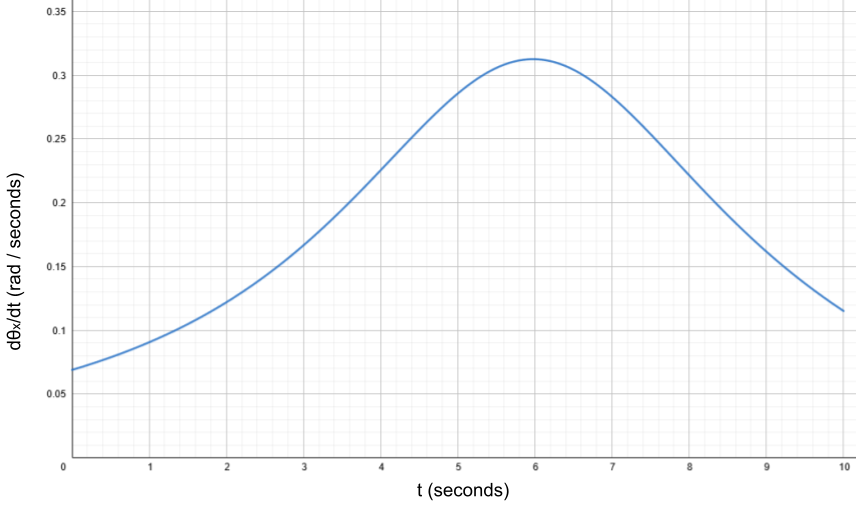
\includegraphics[width=450pt]{img/graph1.png}
\caption{\label{fig:4}Graph of $\dfrac{d\theta_x}{dt}$ vs time $t$}
\end{figure}

The rate of change is far more complex than I previously anticipated. However, this graphical representation reveals far more about the behavior of $\dfrac{d\theta_x}{dt}$ than the algebraic solution. Notice how the angle is strictly increasing since the rate of change is strictly positive as the zipliner is moving in a straight line, meaning that the angle will have to increase to continue viewing it. Moreover, and far more interestingly, the speed of the camera will increase until it reaches an absolute maxima at about 6 seconds, which suggests that the zipliner is closest to the camera at that time. This makes intuitive sense as the camera would have to move the fastest to capture the zipliner as it is closest since any movement is magnified at close distances, then slower when they are farther away (either near the beginning of the zipline or end). However, I wanted to verify that my graphical interpretation was correct by finding the time at which the zipliner is closest to the camera. The distance between the zipliner and camera is shortest when the line of the zipliner is perpendicular to the vector of the camera to the zipliner, solved below.


$$
\begin{array}{c|c}
    \begin{pmatrix} tv_x \\ tv_y \\ tv_z \\ \end{pmatrix} \cdot \begin{pmatrix} x_i+tv_x \\ y_i +tv_y \\ z_i+tv_z \\ \end{pmatrix} = \mid \overrightarrow{P_iP_c} \mid \mid \overrightarrow{CP_c} \mid \cos 90^{\circ} & \text{(Perpendicular hence scalar product 0)}\\ \\
    (v_x^2+v_y^2+v_z^2)t^2 + (v_xx_i+v_yy_i+v_zz_i)t = 0 & \text{(Evaluate \& factorize)}\\ 
    t\left[(v_x^2+v_y^2+v_z^2)t + (v_xx_i+v_yy_i+v_zz_i)\right] = 0 & \text{(Factorize t)}\\ 
    t = -\dfrac{v_xx_i+v_yy_i+v_zz_i}{v_x^2+v_y^2+v_z^2}& \text{(Solve for t} \neq 0 \text{)}\\ \\
    t = -\dfrac{-5.2(24) - 2(28) - 1.1(11)}{5.2^2+2^2+1.1^2} \approx 5.98 \text{ seconds}& \text{(Substitute values in)}
\end{array} 
$$

As expected, the camera is closest to the zipliner at around 6 seconds, meaning that we correctly graphically interpreted the meaning of the maximum rate of change! I find it interesting how only by combining graphing and algebraic vector operations could we understand how the camera rotates the fastest as the zipliner is closest to it. Similarly, let's graph $\frac{d\theta_y}{dt}$ across time. 

\begin{figure}[H]
\centering
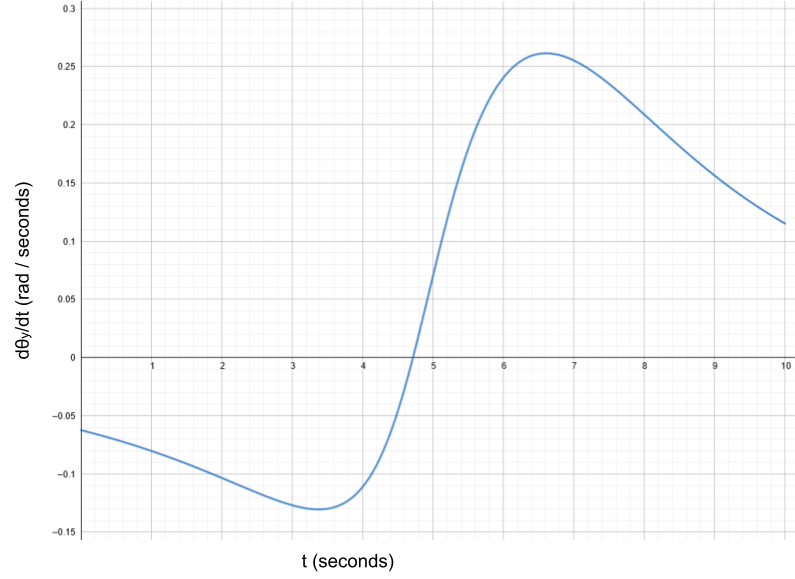
\includegraphics[width=400pt]{img/graph2.png}
\caption{\label{fig:5}Graph of $\dfrac{d\theta_y}{dt}$ vs time $t$}
\end{figure}

This is my favorite graph of the two because of how complex the rate of change appears to be. There is an absolute minima, where the camera is rotating the fastest in the opposite direction, and maxima, where it is rotating in the positive direction. This shocked me because initially, I was expecting all the angles to always be increasing, meaning that the rates of change would all have positive values. This is not necessarily the case, as shown with the rotation about the $\vec j$ orthogonal vector, as this motor would have to compensate for the rotation done by the motor rotating about the $\vec i$ orthogonal vector and counter-intuitively decrease at first. This demonstrates the sophistication of this investigation, because even something as simple as tracking a zipliner for high-quality videos is extremely complex when considered in three dimensions. Despite the zipliner traveling in a straight line (this fooled me into expecting a simple rate of change), $\theta_y$ is not strictly increasing as a consequence of the rotation done by $\theta_x$. 

Given how surprising the negative of the rate of change was, I wanted to further understand how $\theta_y$ will graphically appear, so I graphed $\theta_y$ in degrees so that it can be easily interpreted by the human eye.

\begin{figure}[H]
\centering
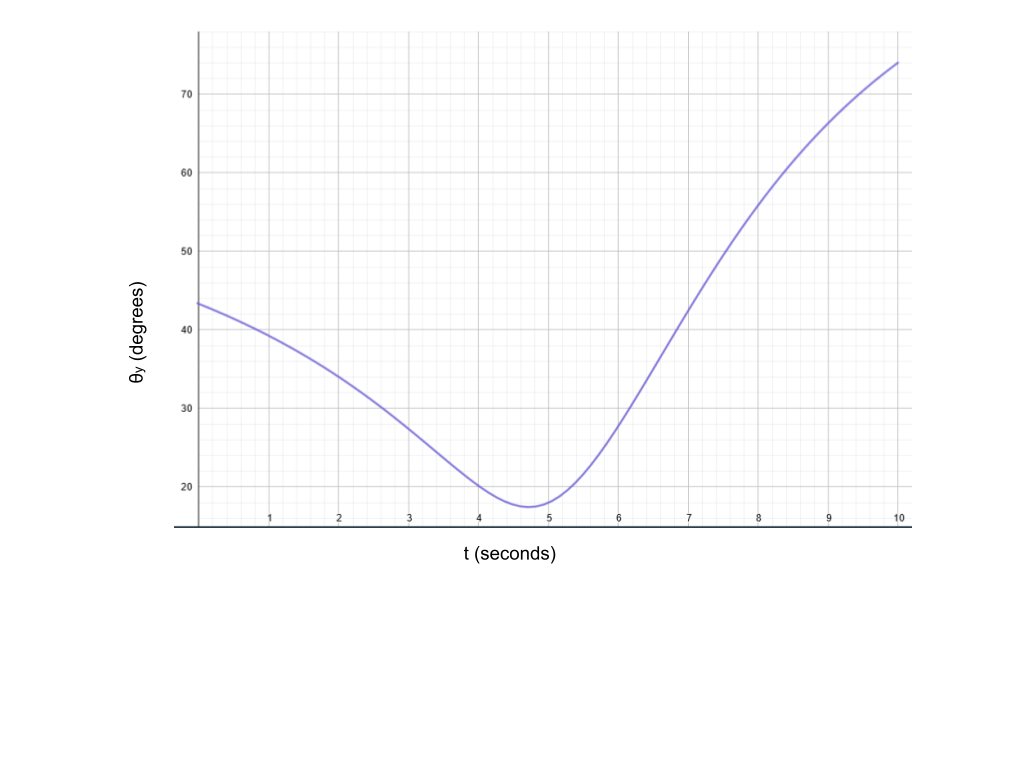
\includegraphics[width=500pt]{img/minigraph.png}
\vspace{-80pt}
\caption{\label{fig:6}Graph of $\theta_y$ vs time $t$}
\end{figure}

As predicted by the negative rate of change, the angle initially decreases until about $4.7$ seconds, the exact same time at which $\dfrac{d\theta_y}{dt}$ is equal to zero, at which point the angle begins rotating in the positive direction and increasing. I really enjoyed this detail about the angles because it demonstrates how 3D rotations easily fool human intuition about orientation. I myself admit to being pleasantly surprised by this counter-intuitive rotation! 


\section{Conclusion}
The rates of change for the two angles defining the orientation of the camera to capture the zipliner as they travel down the zipline were successfully derived through a mixture of related rates calculus and 3-dimensional vectors. What was most fascinating about the results is that even though the zipliner moves in a straight line at constant velocity, the angles do not exhibit linear rotation, rather have far more complex behavior since they are affected by changes in position in the three dimensions. The final results were both shocking due to their complexity and pleasing because of the beauty in their insight into vector calculus. As intimidating as the evaluated equations in terms of time are, their vector form has striking, unexpected similarity. It is also interesting how the two angles have similar equations for their rates of change yet differ so drastically when viewed graphically, demonstrating both a pattern and discrepancy in the behavior of each motor's rotation.
\subsection{Strengths}

A particular strength of this investigation is the use of vectors when finding the related rates. This allowed for the camera to be oriented in three dimensions, which is especially helpful for tracking any real-world objects which are not limited to two dimensional movement. 

Moreover, the equations derived for each angle and their rate of change can be used for any camera and zipline setup without restrictions to where it should be positioned. This is especially helpful if some tourists want a video with a mountain in the background or the river; simply modify the coordinates of point $C$. Similarly, any zipline can be evaluated regardless of its size by modifying coordinates $P_i$ and $P_f$. 

\subsection{Limitations}
The biggest limitation of this investigation is that it assumes the zipliner is traveling at constant velocity. This approximates the motion of a zipliner over time because high frictional forces result in the zipliners achieving terminal velocity that can be used as $\vec v$ \autocite{terminal}. However, gravity still plays a role in accelerating the zipliner as they travel, especially in the first few seconds of the descent. This results in the time axis in reality slightly deviating from my calculations, however, it has no effect on the overall behavior of the angles and their rates of change, only scales the time axis. 

% SOURCE; https://phys.libretexts.org/Courses/Joliet_Junior_College/Physics_201_-_Fall_2019/Book%3A_Physics_(Boundless)/6%3A_Applications_of_Newton/6.07%3A_Drag_Force_and_Terminal_Speed

\subsection{Extensions and Improvements}
An extension that was hinted at throughout the investigation was to instead use vector calculus to find the angles and their rates of change. This would provide more insight into the equations and the reason behind each variable. For example, if I created an angle-vector for angles $\theta_x$ and $\theta_y$, while in reality this would have no real-world meaning, it would showcase the the angles live in a unit sphere that Euler used to develop the concept of Euler Angles \autocite{euler}. 

Additionally, I would love to find the rates of change without constant velocity so that the camera always captures the zipliner in the center of the frame, even when accelerating. This extension would incorporate the acceleration vector into the equations which would undoubtedly make them more complex \autocite{acceleration}. 

\vspace{30pt}

This camera setup will make countless tourists at my Uncle's zipline park happy with unforgettable memories as their paralyzing fear of descending large ziplines is forever recorded for them to watch! Why use bad-quality smartphone videos if you can use 3D vectors and calculus instead?!

\newpage
\printbibliography

\end{document}
